%%%%%%%%%%%%%%%%%%%%%%%%%%%%%%%%%%%%%%%%%%%%%%%%%%%%%%%%%%%%%%%%%%
%
% Analysis of Algorithms
%
% Homework Assignment #5
%
%%%%%%%%%%%%%%%%%%%%%%%%%%%%%%%%%%%%%%%%%%%%%%%%%%%%%%%%%%%%%%%%%%
%%%%%%%%%%%%%%%%%%%%%%%%%%%%%%%%%%%%%%%%%%%%%%%%%%%%%%%%%%%%%%%%%%
%
% Score Card and Answer Sheets
%
%%%%%%%%%%%%%%%%%%%%%%%%%%%%%%%%%%%%%%%%%%%%%%%%%%%%%%%%%%%%%%%%%%
\documentclass[addpoints,11pt]{exam}
\usepackage{clrscode4e}
\usepackage{tcucosc}
\usepackage{units}
\usepackage{enumitem}
\usepackage{hyperref}
\usepackage{fullpage}


%%%%%%%%%%%%%%%%%%%%%%%%%%%%%%%%%%%%%%%%%%%%%%%%%%%%%%%%%%%%%%%%%%
%
% Begin Document
%
%%%%%%%%%%%%%%%%%%%%%%%%%%%%%%%%%%%%%%%%%%%%%%%%%%%%%%%%%%%%%%%%%%
\begin{document}
\pagestyle{empty}


\noindent{\large\bfseries Name: Zachary Macadam}\\
\noindent{\large\bfseries COSC 40403 - Analysis of Algorithms: Homework 5}\\
\noindent{\large\bfseries Due: 23:59:59 on November 6}

%%%%%%%%%%%%%%%%%%%%%%%%%%%%%%%%%%%%%%%%%%%%%%%%%%%%%%%%%%%%%%%%%%
%
% Score Card and Answer Sheets
%
% Comment out one-or-the-other to show or not-show the answers.
%
%%%%%%%%%%%%%%%%%%%%%%%%%%%%%%%%%%%%%%%%%%%%%%%%%%%%%%%%%%%%%%%%%%
\printanswers
%%\noprintanswers


%%%%%%%%%%%%%%%%%%%%%%%%%%%%%%%%%%%%%%%%%%%%%%%%%%%%%%%%%%%%%%%%%%
%
% Score Card
%
%%%%%%%%%%%%%%%%%%%%%%%%%%%%%%%%%%%%%%%%%%%%%%%%%%%%%%%%%%%%%%%%%%
\ifprintanswers
\noindent
\begin{center}
	\gradetable[v][questions]
\end{center}
\newpage
\fi

%%%%%%%%%%%%%%%%%%%%%%%%%%%%%%%%%%%%%%%%%%%%%%%%%%%%%%%%%%%%%%%%%%
% Question
%%%%%%%%%%%%%%%%%%%%%%%%%%%%%%%%%%%%%%%%%%%%%%%%%%%%%%%%%%%%%%%%%%
\begin{questions}


%%%%%%%%%%%%%%%%%%%%%%%%%%%%%%%%%%%%%%%%%%%%%%%%%%%%%%%%%%%%%%%%%%
% Question
%%%%%%%%%%%%%%%%%%%%%%%%%%%%%%%%%%%%%%%%%%%%%%%%%%%%%%%%%%%%%%%%%%
\question[5] Exercise 22.1-1:  Given an adjacency-list representation of a directed graph, how long does it take to compute the out-degree of every vertex?  How long does it take to compute the in-degree?
\begin{solutionorbox} \\ 
	As seen in the textbook, in an adjacency-list representation there is no quicker way to determine whether a given edge (u, v) is present in the graph than to search for v in the adjacency list Adj[u]. So, the out-degree of a vertex u is equal to the length of Adj[u], and the sum of the lengths of all the adjacency lists in Adj is $|$E$|$. This means that the time to compute the out-degree is $\Theta$(V+E). \\
	The in-degree of a vertex u is equal to the number of times it appears in all the lists of Adj. To search all the lists for each vertex, it would take $\Theta$(V E) time. \\ 
	As the textbook suggests, we can use more memory to decrease the time needed. One solution is to use an array of size $|$V$|$ to count the number of times a vertex appears in the list. The counts in the array represent the in-degree of each vertex. This makes the search $\Theta$(V + E) time with $\Theta$(V) extra space needed.
\end{solutionorbox}

\ifprintanswers
\newpage
\else
\bigskip
\fi



%%%%%%%%%%%%%%%%%%%%%%%%%%%%%%%%%%%%%%%%%%%%%%%%%%%%%%%%%%%%%%%%%%
% Question
%%%%%%%%%%%%%%%%%%%%%%%%%%%%%%%%%%%%%%%%%%%%%%%%%%%%%%%%%%%%%%%%%%
\question[5] Exercise 22.1-2: Give an adjacency-list representation for a complete binary tree with 7 vertices.  Give an equivalent adjacency-matrix representation.  Assume that vertices are numbered from 1 to 7 as in a binary heap.
\begin{solutionorbox} \\ 
	Using a min heap:\\
	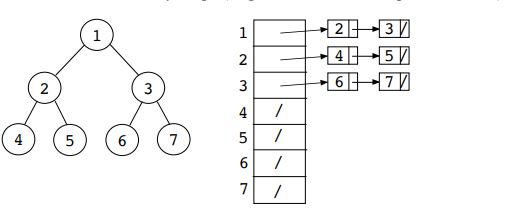
\includegraphics[width=0.5\textwidth]{adjlist.JPG}
\end{solutionorbox}

\ifprintanswers
\newpage
\else
\bigskip
\fi


%%%%%%%%%%%%%%%%%%%%%%%%%%%%%%%%%%%%%%%%%%%%%%%%%%%%%%%%%%%%%%%%%%
% Question
%%%%%%%%%%%%%%%%%%%%%%%%%%%%%%%%%%%%%%%%%%%%%%%%%%%%%%%%%%%%%%%%%%
\question[5] Exercise 22.1-6: Most graph algorithms that take an adjacency-matrix representation as input require time $\Omega(V^2)$, but there are some exceptions.  Show how to determine whether a directed graph $G$ contains a \textbf{\textit{universal sink}} (a vertex with in-degree $\abs{V}-1$ and out-degree 0) in time $O(V)$, given an adjacency matrix for $G$.
\begin{solutionorbox} \\
	By definition, there can be 0 or 1 universal sinks in an adjacency-matrix. If a vertex is a universal sink there are no edges going out of that node and all vertices have edges to it. In an adjacency-matrix representation this means that the row of the universal sink vertex will have all zeroes and the column will have all ones except at the diagonal. If we find the row, denoted i, with all zeroes, we can traverse the column, denoted j, for the corresponding vertex in $O(V)$ time to see if it contains all ones except for when $i = j$. If this is the case, the vertex is a universal sink, otherwise no universal sink exists. The algorithm stops running when a row of all zeros is identified and the column is checked to see if that vertex is a universal sink or not. This shows that a universal sink can be identified in $O(V)$ time. \\ \\
	A method to achieve this result is to remove the vertices that cannot be universal sinks until we are left with one potential universal sink. When we are analyzing a cell $A(i,j)$ where $i \neq $ j, if $A(i,j) = 1$, it means that $i$ has an edge to $j$ and cannot be a sink, else if $A(i,j) = 0$ then vertex $i$ does not have an edge to $j$ and $j$ cannot be a universal sink. We can check all vertices in $n - 1$ time and when we are left with one vertex, we can check its row for zeroes and column for ones in $2n - 1$ time (because we do not need to check the vertex itself). This shows that the algorithm is $O(n - 1 + 2n - 1)$ or $O(n)$ time. 
\end{solutionorbox}

\ifprintanswers
\newpage
\else
\bigskip
\fi


%%%%%%%%%%%%%%%%%%%%%%%%%%%%%%%%%%%%%%%%%%%%%%%%%%%%%%%%%%%%%%%%%%
% Question
%%%%%%%%%%%%%%%%%%%%%%%%%%%%%%%%%%%%%%%%%%%%%%%%%%%%%%%%%%%%%%%%%%
\question[5]
The BFS algorithm listed on page 595 of our textbook and presented in class uses a queue as the data structure for storing discovered vertices.  What happens if you change the data structures to use a stack instead (Be specific)?  Use the example graph on page 596 to demonstrate your solution.   
\begin{solutionorbox}\\
	If we were to replace the queue used in BFS to a stack, the algorithm implemented would resemble DFS instead. The distance array returned would not appropriately derive the distance from the source node, because stack does not allow all the nodes of the same level to "finish", it only allows one. This can be seen clearly in the example below when the search reaches node $t$. Instead of allowing node $x$ to find undiscovered adjacent nodes, the modified algorithm continues to node $u$ giving node $y$ an incorrect distance of 4. This shows that using a stack finds the deepest node when there are more than one node in the same level. Using Figure 22.3 as an Example: \\
	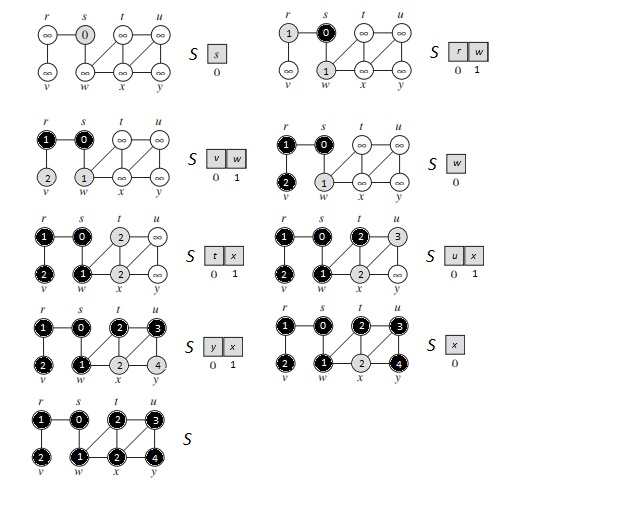
\includegraphics[width=1\textwidth]{bfsstack.jpg}
	
\end{solutionorbox}
	
\ifprintanswers
\newpage
\else
\bigskip
\fi



%%%%%%%%%%%%%%%%%%%%%%%%%%%%%%%%%%%%%%%%%%%%%%%%%%%%%%%%%%%%%%%%%%
% Question
%%%%%%%%%%%%%%%%%%%%%%%%%%%%%%%%%%%%%%%%%%%%%%%%%%%%%%%%%%%%%%%%%%
\question[5] Exercise 22.2-7:  There are two types of professional wrestlers: ``babyfaces'' (``good guys'') and ``heels'' (``bad guys'').  Between any pair of professional wrestlers, there may or may not be a rivalry.  Suppose we have $n$ professional wrestlers and we have a list of $r$ pairs of wrestlers for which there are rivalries.  Give an $O(n+r)$-time algorithm that determines whether it is possible to designate some of the wrestlers as babyfaces and the remainder as heels such that each rivalry is between a babyface and a heel.  If it is possible to perform such a designation, your algorithm should produce it.
\begin{solutionorbox} \\
	To determine if a designation is possible, create a Graph where each vertex is a wrestler and each edge is a rivalry. The graph contains $n$ (number of wrestlers) vertices and $r$ (number of rivalries) edges. \\
	We begin by performing BFS as many times as needed to compute the distances for each vertex. For the designation to be correct, we know that no two babyfaces and no two heels may be rivals (connected in the graph). We can then choose all even numbered distance values to be babyfaces and all odd numbered distance values to be heels (or vice versa, the parity assigned is not important, it is simply used for verifying the rivalries). \\
	We must now check each edge to verify that it goes from a babyface to a heel, if each edge is correct, a designation is possible. \\
	We know that BFS time complexity is $O(V + E)$, so in this case it will be $O(n + r)$. \\
	Designating each wrestler to a babyface or heel takes $O(n)$ time because we do it for each vertex, and verifying that each edge is correct takes $O(r)$ time for r edges. \\
	Since each step of the algorithm takes linear time, we can conclude by choosing the largest linear value that the algorithm takes $O(n + r)$ time to calculate if such a designation is possible.
\end{solutionorbox}

\ifprintanswers
\newpage
\else
\bigskip
\fi



%%%%%%%%%%%%%%%%%%%%%%%%%%%%%%%%%%%%%%%%%%%%%%%%%%%%%%%%%%%%%%%%%%
% Question
%%%%%%%%%%%%%%%%%%%%%%%%%%%%%%%%%%%%%%%%%%%%%%%%%%%%%%%%%%%%%%%%%%
\question[5]
Exercise 22.3-2:  Show how the depth-first search works on the graph of Figure 22.6.  Assume that the \textbf{for} loop of lines 5-7 of the DFS procedure considers the vertices in alphabetical order, and assume that each adjacency list is ordered alphabetically.  Show the discovery time and finishing times for each vertex, and show the classification of each edge.
\begin{solutionorbox} \\ 
	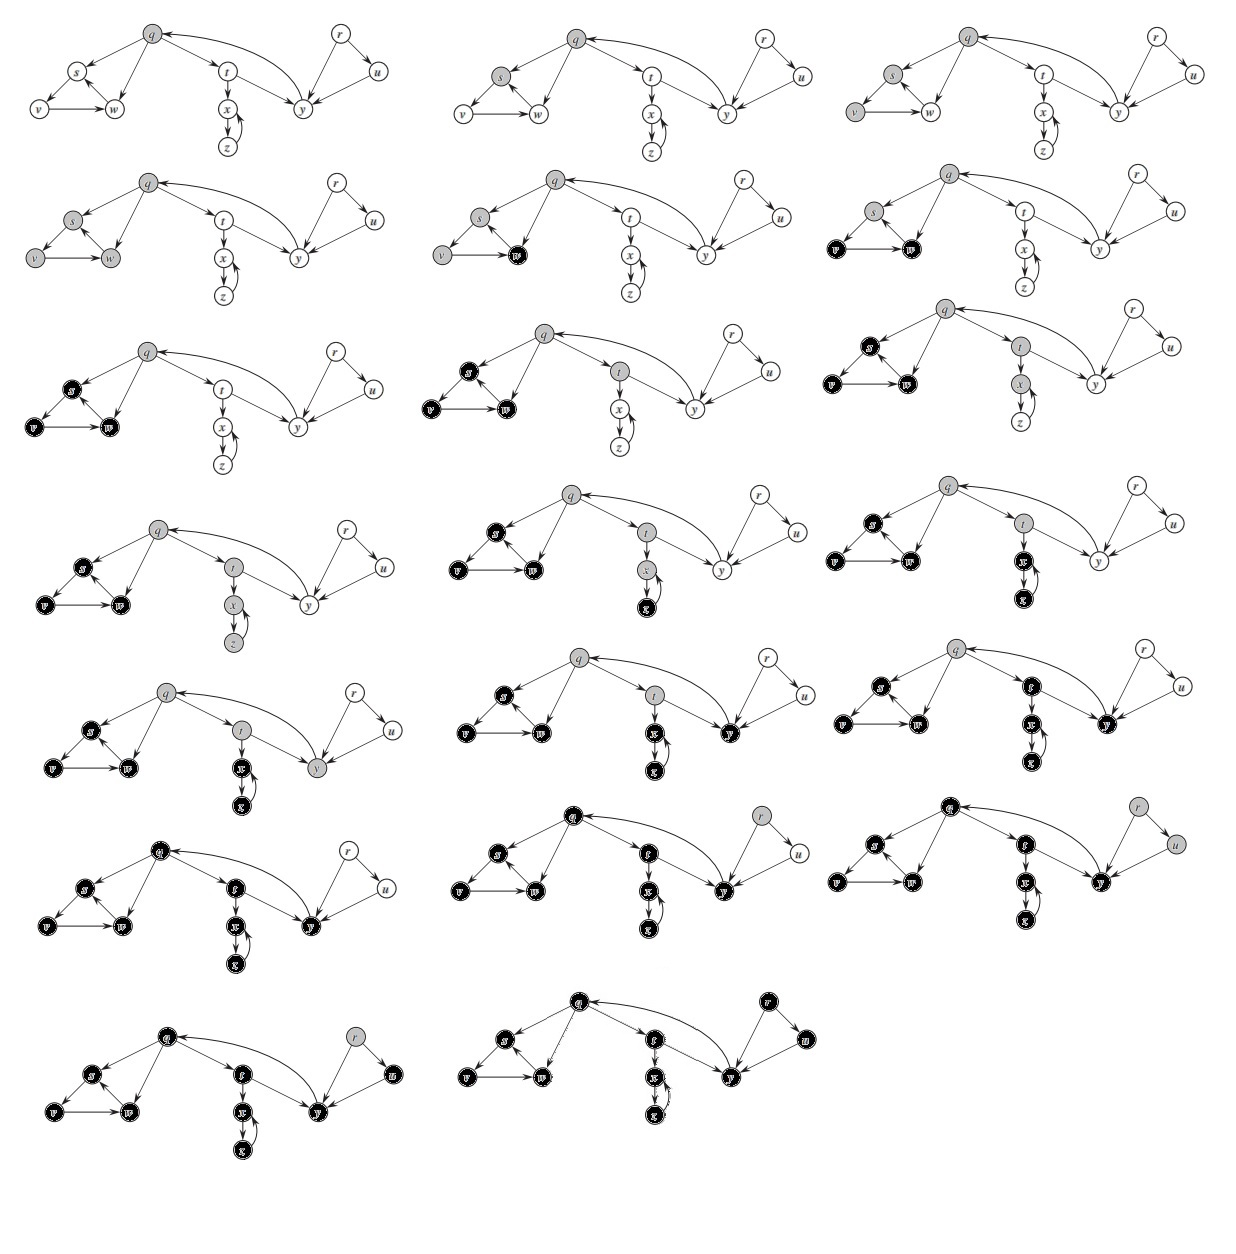
\includegraphics[width=15cm,height=13cm]{dfs.jpg} \\
	\begin{tabular}{c | c | c | c | c | c | c | c | c | c | c}
	     Vertex & q & r & s & t & u & v & w & x & y & z\\
	     \hline
	     Discovery Time & 1 & 17 & 2 & 8 & 18 & 3 & 4 & 9 & 13 & 10\\
	     \hline
	     Finishing Time & 16 & 20 & 7 & 15 & 19 & 6 & 5 & 12 & 14 & 11\\
	\end{tabular} \\ 
	Tree Edges: (q,s), (s,v), (w,w), (q,t), (t,x), (x,z), (t,y), r,u)\\
	Back Edges: (w,s), (z,x), (y,q)\\
	Forward Edges: (q,w)\\
	Cross Edges: (r,y), (u,y)
\end{solutionorbox}

\ifprintanswers
\newpage
\else
\bigskip
\fi



%%%%%%%%%%%%%%%%%%%%%%%%%%%%%%%%%%%%%%%%%%%%%%%%%%%%%%%%%%%%%%%%%%
% Question
%%%%%%%%%%%%%%%%%%%%%%%%%%%%%%%%%%%%%%%%%%%%%%%%%%%%%%%%%%%%%%%%%%
\question[5]
Exercise 22.4-1: Show the ordering of vertices produced by $\proc{Topological-Sort}$ on the dag of Figure 22.8, under the assumption of Exercise 22.3-2.  
\begin{solutionorbox} \\ 
    By performing DFS on the dag in Figure 22.8, we get the following discovery and finishing times: \\ \\
    \begin{tabular}{c | c | c | c | c | c | c | c | c | c | c | c | c | c | c}
        Vertex & m & n & o & p & q & r & s & t & u & v & w & x & y & z \\
        \hline
        Discovery Time & 1 & 21 & 22 & 27 & 2 & 6 & 23 & 3 & 7 & 10 & 11 & 15 & 9 & 12 \\
        \hline
        Finishing Time & 20 & 26 & 25 & 28 & 5 & 19 & 24 & 4 & 8 & 17 & 14 & 16 & 18 & 13 
    \end{tabular} \\ \\
    To obtain an ordering by Topological Sort, we can order the vertices in descending order of finishing time to get the following: \\
    $p, n, o, s, m, r, y, v, x, w, z, u, q, t$
\end{solutionorbox}

\ifprintanswers
\newpage
\else
\bigskip
\fi




\end{questions}
\end{document}
